\documentclass[12pt]{article}

\usepackage{fontawesome}
\usepackage{hyperref}
\usepackage{xurl}
\usepackage{graphicx}
\usepackage{float}
\usepackage[tagged, highstructure]{accessibility}
\usepackage{bookmark}
\usepackage{enumitem}

\hypersetup{
    colorlinks=false,
    pdfborder={0 0 0},
    pdftitle={Data Integrity Lab},
    pdfauthor={Adrianna Holden-Gouveia},
    pdfsubject={Introduction to Data - Lab Assignment},
    pdflang={en-US},
    pdfkeywords={data integrity, data quality, data validation, machine learning}
}

% Configure PDF bookmarks for navigation
\bookmarksetup{
    numbered,
    open,
}

% Configure list spacing for better accessibility
\setlist{nosep}


\title{Data Integrity}
\author{
        Adrianna Holden-Gouveia \\
        Website: \href{https://aholdengouveia.name}{aholdengouveia.name}\\ 
        \date{\vspace{-5ex}}
        %Email: \href{mailto:admin@aholdengouveia.name}{admin@aholdengouveia.name} \\
%        \faLinkedin{: aholdengouveia} \\
        \faGithub {: aholdengouveia} \\
        %\faTwitter {: aholdengouveia} \\
        }

%S\date{\today}


\begin{document}    

\maketitle

%\begin{abstract}
%\end{abstract}
%\tableofcontents


\section*{Accessibility Notice}
This document is also available in HTML format at:

Link: \href{https://aholdengouveia.name/IntroData/labs/dataintegrity.html}{\textbf{\nolinkurl{https://aholdengouveia.name/IntroData/labs/dataintegrity.html}}}

The HTML version provides enhanced accessibility features including keyboard navigation, screen reader support, responsive design, dark mode support, and high contrast options.

\section*{Learning Outcomes}
By the end of this lab, you will be able to:
\begin{itemize}
    \item Identify data integrity issues such as outliers, inconsistent formatting, extra whitespace, and duplicates
    \item Use data cleanup tools in Google Sheets to fix issues in a data set
    \item Explain what likely went wrong when data was collected
    \item Use a machine learning tool to predict values, and describe the results
\end{itemize}

\section*{Lab Instructions}


To do this lab you need:
\begin{itemize}
    \item The HalloweenCandy.csv data set, linked here Link: \href{https://www.aholdengouveia.name/IntroData/labs/HalloweenCandy.csv}{\textbf{\nolinkurl{https://www.aholdengouveia.name/IntroData/labs/HalloweenCandy.csv}}}
    \item The data you collected for the Data Collection lab in Week 2
    \item Google Sheets with the Simple ML for Sheets extension. If you do not have a Google account, you can get one for free before doing this lab.
\end{itemize}

Before attempting this lab, watch this video on Simple ML for Sheets to get an idea of what can be done with Machine Learning Link: \href{https://www.youtube.com/watch?v=GYCORMNr_IU}{\textbf{\nolinkurl{https://www.youtube.com/watch?v=GYCORMNr_IU}}}

The documentation for Google Sheets is linked under Resources.

\subsection*{Screenshots}
Several questions ask for a screenshot. Each screenshot should have your name, term, and year.  One of the easiest ways to do that is make a text document with your name and term/year on your computer and save it to use all term. Any screenshots that don't include this information won't be counted.

\begin{figure}[H]
    \centerline{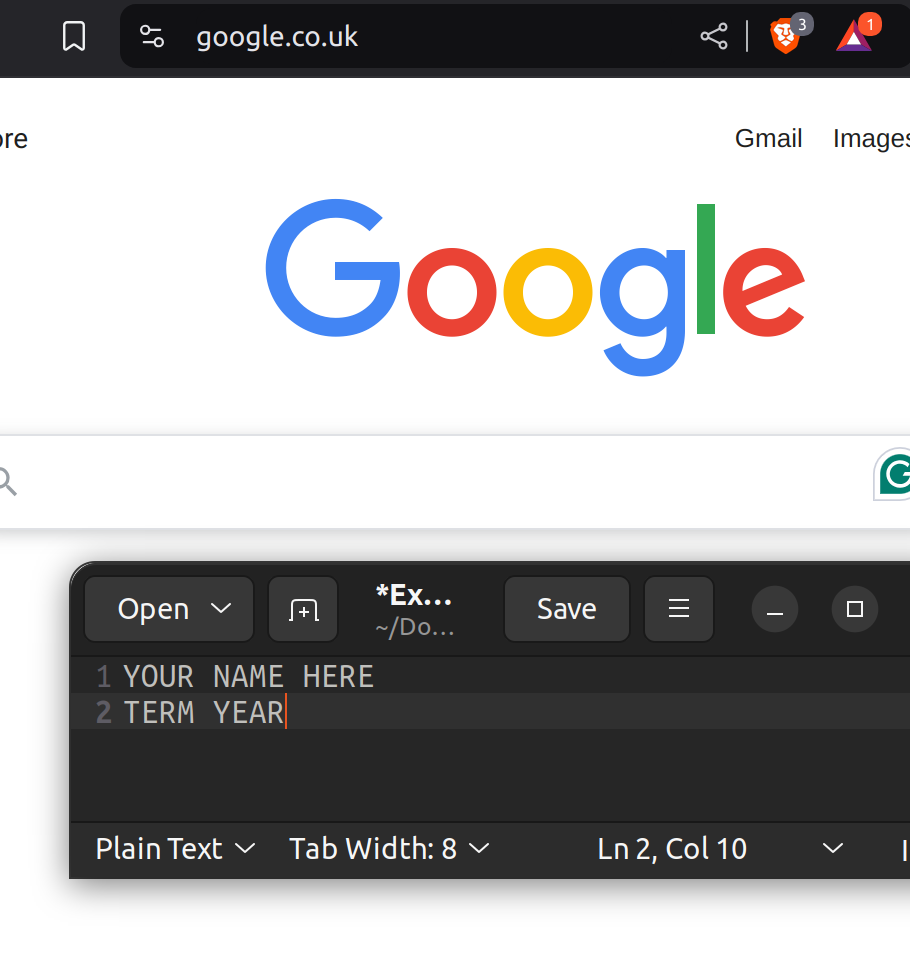
\includegraphics[scale=.2]{ExampleScreenshot.png}}
    \caption{This is an image of what each of your screenshots should look like}
    \alt{Example screenshot: a web browser showing the Google home page, with a small text editor window in front of it that says YOUR NAME HERE and TERM YEAR}
    \end{figure}

\section*{Given Data set}
Using the given data set HalloweenCandy.csv, we're going to actively explore the dataset and look for potential issues, including missing data, inconsistent formatting, duplicates, or outliers. The tools we'll be using are going to be under Data and Extensions in Google Sheets.

Open the data set in Google Sheets, try the data tools, and answer the following questions.

\textbf{Note:} the duplicate tool removes the duplicates it finds. For question 3, write down how many duplicates it found, then undo it before you do question 4.
\begin{enumerate}
    \item Age and country (the Q3: AGE and Q4: COUNTRY columns)
    \begin{enumerate}
        \item Looking at Q3: AGE, do you see any outliers or things that look different than you expected? For example, did everyone enter a number for their age? If not, what did they enter?
        \item What do you think went wrong in the collection of that data?
        \item Looking at Q4: COUNTRY, what did you notice? What do you think went wrong?
    \end{enumerate}
    \item Whitespace
    \begin{enumerate}
        \item Trim the whitespace. How much whitespace did you get rid of?
        \item Visually, what changed in your data?
    \end{enumerate}
    \item Using the duplicate check on the whole sheet, how many duplicates are there? Take a screenshot.
    \item Using the duplicate check on the whole sheet except the Internal ID column, how many duplicates are there? Take a screenshot.
    \item Cleanup suggestions
    \begin{enumerate}
        \item What are the suggested actions to take?
        \item What happened after you did them?
    \end{enumerate}
    \item Column stats. After doing the cleanup suggestions, review the column stats and pick one column to look at the suggested graph.
    \begin{enumerate}
        \item What column did you pick? Why?
        \item What's going on in the graph?
        \item Take a screenshot of the graph.
    \end{enumerate}
    \item Simple ML for Sheets. Try predicting values on two columns: the Q3: AGE column and one column of your choice.
    \begin{enumerate}
        \item Which other column did you pick? Why?
        \item How did it work? What happened?
        \item How long did it take?
        \item Take a screenshot of your results.
    \end{enumerate}
\end{enumerate}

\section*{Your data set}
Using the data you collected for the Data Collection lab in Week 2, we're going to explore how we can check over that data for potential issues.  You can choose to do more data validation than what's listed here, but make sure to note that in your documentation.

Open your data set in Google Sheets, try the data tools, and answer the following questions.
    \begin{enumerate}
        \item Outliers
        \begin{enumerate}
            \item Pick two of the columns. Which columns did you pick to check, and why?
            \item Do you see any outliers or things that look different than you expected?
        \end{enumerate}
        \item Whitespace
        \begin{enumerate}
            \item Trim the whitespace. How much whitespace did you get rid of?
            \item Visually, what changed in your data?
        \end{enumerate}
        \item Using the duplicate check on the whole sheet, how many duplicates are there? Take a screenshot.
        \item Cleanup suggestions
        \begin{enumerate}
            \item What are the suggested actions to take?
            \item What happened after you did them?
        \end{enumerate}
        \item Column stats. After doing the cleanup suggestions, review the column stats and pick one column to look at the suggested graph.
        \begin{enumerate}
            \item What column did you pick? Why?
            \item What's going on in the graph?
            \item Take a screenshot of the graph.
        \end{enumerate}
        \item Simple ML for Sheets. Try predicting values on two of the columns.
        \begin{enumerate}
            \item Which two columns did you pick? Why?
            \item How did it work? What happened?
            \item How long did it take? Were you expecting it to take more or less time than it did?
            \item Take a screenshot of your results.
        \end{enumerate}
    \end{enumerate}

\section*{Deliverables}
\begin{enumerate}
    \item A text document with the answers to the questions for the given data on Halloween Candy, labeled with their question numbers.
    \item A text document with the answers to the questions for your data set, labeled with their question numbers.
    \item All screenshots, clearly labeled: 4 for the Halloween Candy data (questions 3, 4, 6, and 7) and 3 for your data (questions 3, 5, and 6).
    \item Your data as a CSV after you have finished the data cleanup tools and any changes.
\end{enumerate}

\section*{Resources}
References, a video, a PowerPoint and some notes are available at my website
Link: \href{https://www.aholdengouveia.name/IntroData/dataintegrity.html}{\textbf{\nolinkurl{https://www.aholdengouveia.name/IntroData/dataintegrity.html}}}

Google Sheets documentation
Link: \href{https://support.google.com/docs/topic/1361472}{\textbf{\nolinkurl{https://support.google.com/docs/topic/1361472}}}

\end{document}